\begin{center}
\begin{longtable}{ |l|l| } 
 \hline
 Attribute & Description\\ 
 \hline
 timestamp & time when session started\\ 
 \hline
 userSessionId & ID of the session\\ 
 \hline
 userId & ID of the user in session\\ 
 \hline
 teamId & ID of the team that user is in\\ 
 \hline
 assignmentId & Temp ID assigned to the user (while in the team/session)\\ 
 \hline
 sessionType & type of the event (start or end)\\ 
 \hline
 teamLevel & level of the team in the current session\\ 
 \hline
 platformType & what device / platform is being used\\ 
 \hline
\caption{user-session.csv}
\end{longtable}
\end{center}

User session dataframe does not have any missing values.
\begin{figure}[H]
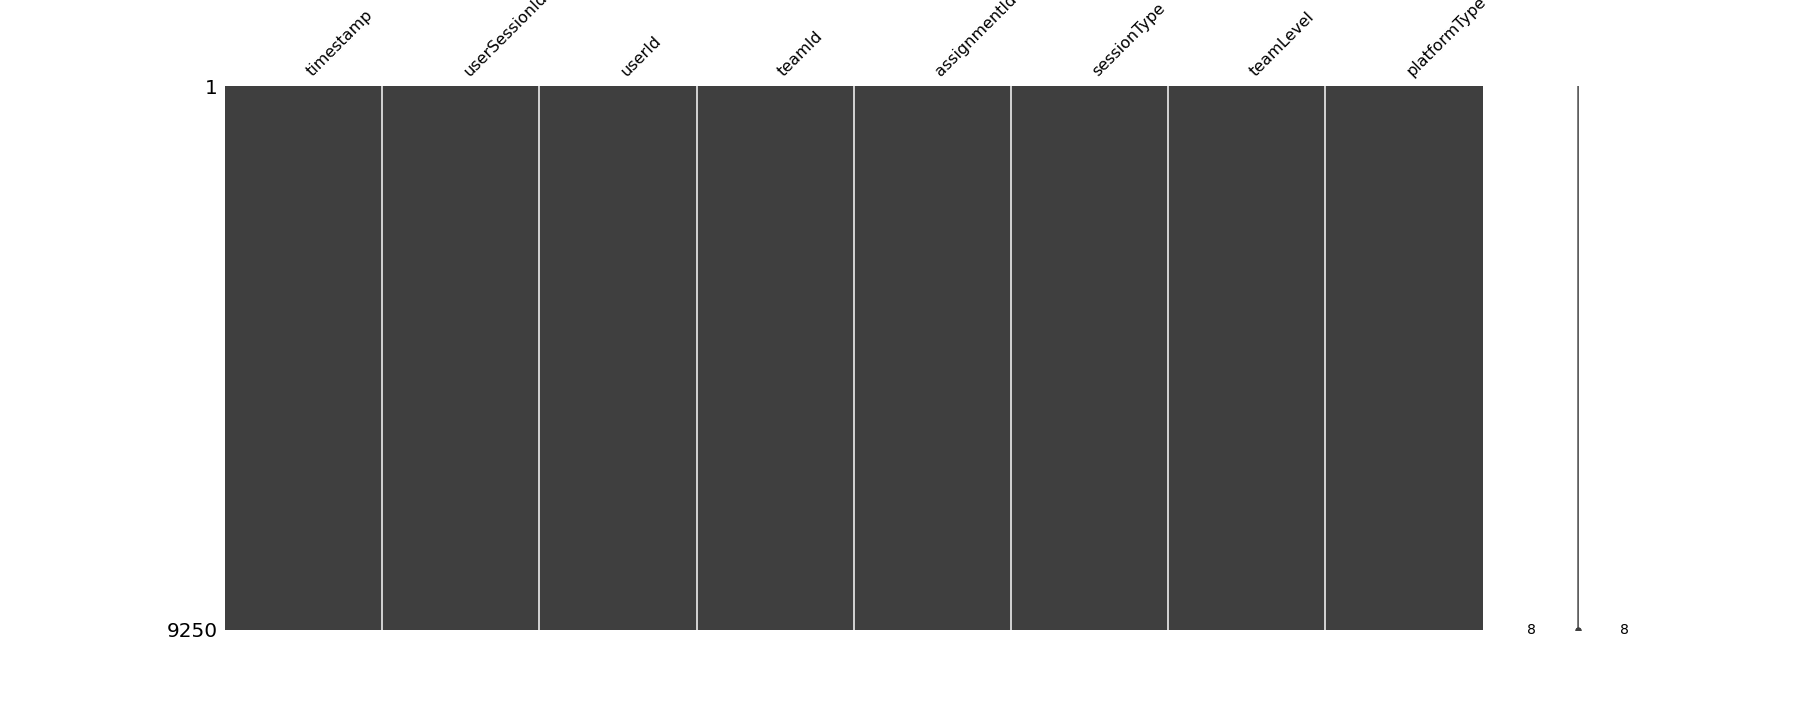
\includegraphics[scale=0.25]{img/Graphs/userSession/missingno_userSession.png}
\centering
\caption{missingno\_userSession}
\label{fig:missingno_userSession}
\end{figure}

Time series for user session appears to be spiky (simmilar to levelEvents, Figure \ref{fig:timeseries_levelEvents}). It ends with the same fall as other time series events.
\begin{figure}[H]
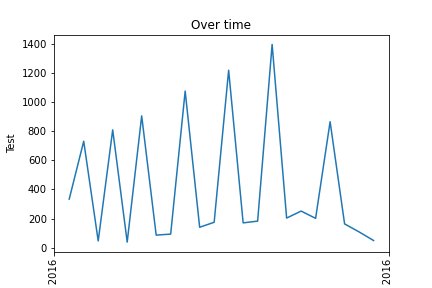
\includegraphics[scale=0.85]{img/Graphs/userSession/timeseries_userSession.png}
\centering
\caption{timeseries\_userSession}
\label{fig:timeseries_userSession}
\end{figure}

If we compare start and end of sessions for platforms, we can see that users tend not to switch platforms while the session is running. This could be one of the game limitations, meaning if you would rejoin from other platform, your session would expire.
\begin{figure}[H]
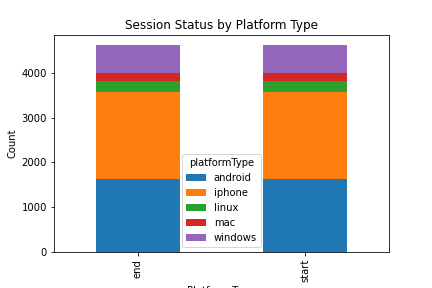
\includegraphics[scale=0.85]{img/Graphs/userSession/histogram_userSession.png}
\centering
\caption{histogram\_userSession}
\label{fig:histogram_userSession}
\end{figure}